\chapter{Interpretation and implications of scaling laws}
\label{chap:scaling_implications}

\bigskip

\section{What scaling laws tell us about cities}

Before concluding this part, it is important to understand what exactly scaling
laws can tell us about cities. Scaling laws are, by essence, cross-sectionnal
studies of cities. As opposed to a dynamical study where one would follow the
evolution of single cities over time, scaling laws tells us about the behaviour
of an \emph{ensemble} of cities at a give point in time. Throughout
Chapters~\ref{chap:scaling_introduction} and~\ref{chap:scaling_model}, we have
implicitely assumed that scaling laws are the signature of phenomena occuring at
the intra-urban level. This assumption, we call \emph{evolution interpretation},
is however not completely obvious. 

The interpretation of allometric scaling laws in Biology is straightforward,
because the compared organisms are independent. Indeed, the mass of a
given elephant at a point in time $t$ is not correlated to the mass of any other
living creature in the world. Therefore, scaling relationships can only be
understood as resulting from the existence  of similar processes in the growth
of these different animals. Cities, on the other hand, are part of a bigger
system -- the system of cities -- and interact constantly through networks.
People change residence, companies relocate, goods are shipped and money is
transfered. Therefore, as argued by Denise Pumain~\cite{Pumain:2012}, scaling
laws can also be construed as reflecting the redistribution processes within the
system of cities. We call this the \emph{differentiation interpretation}.

\subsection{The evolution interpretation}
\label{sub:the_evolution_interpretation}

The evolution interpretation (Figure~\ref{fig:evolution_interpretation}) has
been widely adopted in the scaling literature~\cite{Bettencourt:2007,
Bettencourt:2013,Louf:2014_scaling} without ever being really stated, let alone
justified. It is based on two assumptions. First, that the cities in the dataset
are different realisations of the same system. Thus, as stated in
Chapter~\ref{chap:scaling_introduction}, looking at the scaling of various
quantities with population size is a way to probe the system's internal
processes.

\begin{figure}[!h]
    \centering
    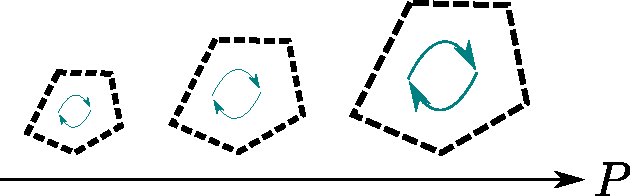
\includegraphics[width=\textwidth]{gfx/chapter-scaling/evolution-interpretation.pdf}
    \caption{{\bf Evolution interpretation.} In this interpretation we consider
    that cities are different realisations of the same system. The intra-urban
processes are responsible for the non-linear scaling of the different
quantities.\label{fig:evolution_interpretation}}
\end{figure}

The second assumption has to do with the time scales over which the different
processes occur. It has indeed been observed that some scaling laws were stable
over time, even though the population of the cities is constantly changing.
This is only possible, however, if the timescale the processes responsible for
the value of the quantity being studied occur over timescales that are at worst
of the same order of the timescales over which population changes. For instance,
an abrupt increase in population size is not likely to be immediately reflected
in terms of the length of streets, while the evolution of the total commuted
length will be almost instantaneous.

If the two previous assumptions are verified, then one can indeed use
transversal scaling relationships as a way to probe the internal dynamics of
cities.\\

As an aside, the previous discussion hints at the difficulty to intepret the
values of the observed deviations to scaling laws~\cite{Bettencourt:2010a}. It is
indeed difficult to assess to what extent they account for a real over
or under-performance of the city compared to the other cities, or
 for the time it takes for the studied quantity to react to population changes.
Unfortunately, we cannot answer these questions until we understand in details
the mechanisms reponsible for the evolution of the corresponding quantities in time.

\subsection{The differentiation interpretation}
\label{sub:the_differentiation_interpretation}

As Denise Pumain judiciously claims~\cite{Pumain:2006,Pumain:2012}, the evolution
interpretation is not the only possible interpretation of scaling laws. In some
cases and the mechanisms responsible for scaling relationships should be sought
after in the hierarchical organisation of cities and their interactions.\\

\begin{figure}[!h]
    \centering
    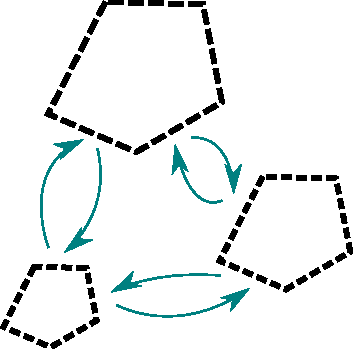
\includegraphics[width=0.5\textwidth]{gfx/chapter-scaling/system-interpretation.pdf}
    \caption{{\bf Differentiation interpretation.} In this interpretation, we
    consider that the redistribution processes occuring within systems of cities
are reponsible for the non-linear scaling of quantities with city size in this
system.\label{fig:label_fig}}
\end{figure}

We briefly mentioned in Chapter~\ref{chap:scaling_model} that allometric scaling relationships
could only be obtained when considering cities belonging to the same system of
cities. The fact that we observe scalings when taking a single country into
account, and a cloud of points when mixing two different countries, is a
signature of the integration of cities into systems of cities. Although it is
not clear at the moment what are the mechanisms reponsible for the
'equilibration' of the scaling there clearly is an adjustement that is being
made, because the economy, the population, etc. are tightly connected through
the flow of commodities, populations, information and funds.\\

Now, the same connections may be responsible for the scaling relationships
themselves. As an example, Pumain et al.~\cite{Pumain:2006} study the scaling of
the number of employees from different economic sector with population size (see
Chapter~\ref{chap:scaling_introduction}.\\

So, are scaling relationships properties of cities, or of systems of cities.
Probably both. The scaling of some quantities, such as the total quantity of
CO\textsubscript{2} emitted or the tota length of roads are undoubtedly due to
intra-urban processes. Others, such as the linear scaling of total income, are
probably due to the interactions of cities within the same system of cities.
However, it is impossible to discriminate between both interpretations on an
empirical basis. Ultimately, models that are able to reproduce 


\section{What cities?}
\label{sec:what_cities_}

\cite{Louf:2014_smog} for problem with the $CO_2$\\
\cite{Arcaute:2014} for variation of exponents with city definition.


The success of natural sciences lies in their great emphasis on the role of
quantifiable data and their interplay with models. Data and models are both
necessary for the progress of our understanding: data generate stylized facts
and put constraints on models. Models on the other hand are essential to
comprehend the processes at play and how the system works. If either is missing,
our understanding and explanation of a phenomenon are questionable. This issue
is very general, and affects all scientific domains, including the study of
cities. \\

Until recently, the field of urban economics essentially consisted in untested
laws and theories, unjustified concepts that supersede empirical
evidence~\cite{Bouchaud:2008}. Without empirical validation, it is not clear
what these models teach us about cities. The tide has turned in recent years,
however: the availability of data is increasing in size and specificity, which
has led to the discovery of new stylized facts and opened the door to a new
science of cities~\cite{Batty:2013}. The recent craze for scaling
laws~\cite{Batty:2008,Bettencourt:2007,Pumain:2004}, for instance, has been an
important new step in the study of urban systems.

These laws present themselves as a power-law relationship between socioeconomic
(GDP, number of patents), structural (length of roads, of cables) quantities
$Y$, and the size of the population $P$ of the city:

\begin{equation}
Y = P^{\, \beta}
\end{equation}


where the exponent $\beta$ can be different from $1$. This type of scaling relation is a signature
of various processes governing the phenomenon under study, especially when the exponent
$\beta$ is not what is naively expected~\cite{Barenblatt:2003}. However, as more and more scaling
relationships are being reported in the literature, it becomes less and less clear what we really
learn from these empirical findings. Mechanistic insights about these scalings are usually
nonexistent, often leading to misguided interpretations.\\

\begin{figure}[!h]
	\centering
	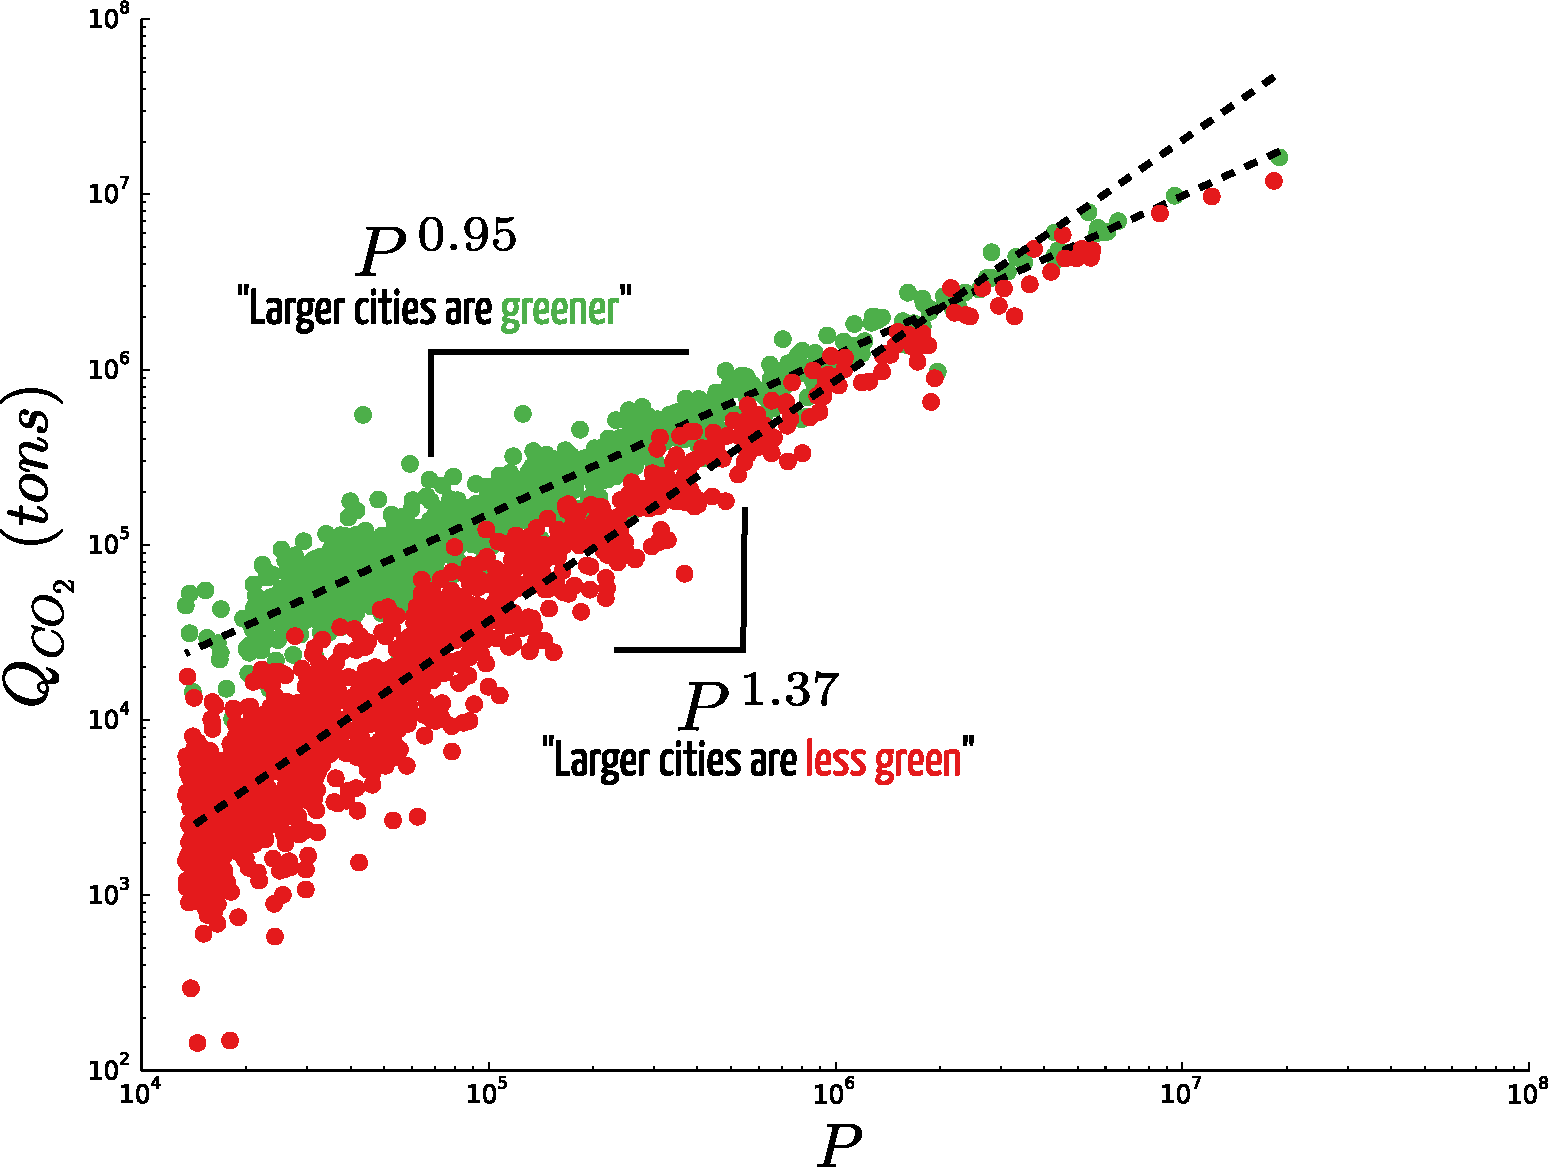
\includegraphics[width=\textwidth]{gfx/chapter-scaling/lost_smog.pdf}
	\caption{ {\bf Are larger cities greener or smoggier?} Scaling of transport-related $CO_2$
emissions with the population size for US cities from the same dataset but at different aggregation
levels. In red, the aggregation is done at the level of urban areas and in green for combined statistical
areas. Depending on the definition of the city, the scaling exponents are qualitatively different, leading
to two opposite conclusions. Data on $CO_2$ emissions were obtained from the Vulcan Project (\url{http://
vulcan.project.asu.ed}) (see~\cite{Fragkias:2013,Oliveira:2014}). Data on the population of urban areas and
metropolitan statistical areas were obtained from the Census Bureau (\protect\url{http://www.census.org}). \label{fig}}
\end{figure}

\begin{figure}
    \centering
    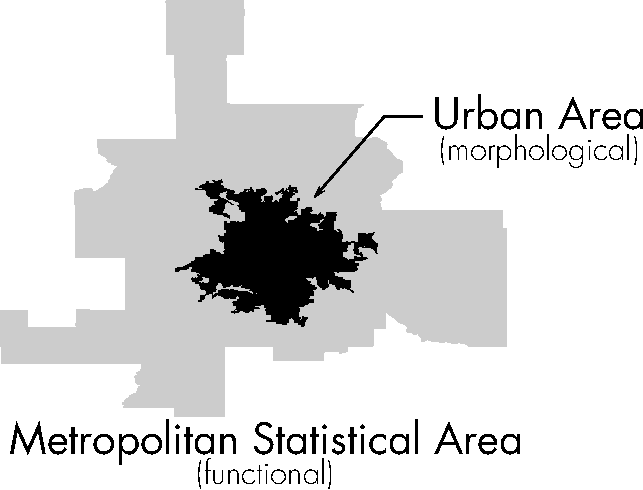
\includegraphics[width=\textwidth]{gfx/chapter-scaling/city_definition.pdf}
    \caption{{\bf City definitions in the US.} The Minneapolis Urban Area (in
    black) is defined by the Census Bureau as contiguous block groups with at
least $1000$ inhabitants per square mile. The Minneapolis-St. Paul Metropolitan
Statistical Area (in grey) is defined as the counties containing the urban area
as well as any adjacent county that have a high degree of integration with the
core, as measured with commuting flows.\label{fig:two_definitions}}
\end{figure}

A striking example of the fallacies which hinder the interpretation and application
of scaling is given by different studies on $CO_2$ emissions due to transportation~\cite{Fragkias:2013,Glaeser:2010,Oliveira:2014,Rybski:2013}. The topic
is particularly timely: pollution peaks occur in large cities worldwide with a seemingly
increasing frequency, and are suspected to be the source of serious health problems~\cite{Bernstein:2004}. Glaeser and Kahn~\cite{Glaeser:2010}, Rybski et al~\cite{Rybski:2013}, Fragkias et al~\cite{Fragkias:2013}, and Oliveira et al~\cite{Oliveira:2014} are interested in how $CO_2$ emissions scale with the population size
of cities. The question they ask is simple: Are larger cities greener---in the sense that there
are fewer emissions per capita for larger cities---or smoggier? Surprisingly, these different
studies reach contradictory conclusions. We identify here two main sources of error which
originate in the lack of understanding of the mechanisms governing the phenomenon.

The first error concerns the estimation of the quantity $Q_{CO_2}$ of $CO_2$ emissions due to
transportation. In the absence of direct measures, Glaeser and Kahn~\cite{Glaeser:2010} have chosen
to use estimations of $Q_{CO_2}$ based on the total distance traveled by commuters. This is in fact
incorrect, and in heavily congested urban areas the relevant quantity is the total time spent
in traffic~\cite{Louf:2013}. Using distance leads to a serious underestimation of
$CO_2$ emissions: the effects of congestion are indeed strongly nonlinear, and the time spent
in traffic jams is not proportional to the traveled distance. As a matter of fact, commuting
distance and time scale differently with population size, and the time spent commuting and
$CO_2$ emissions scale with the same exponent~\cite{Louf:2014}.

The second, subtler, issue lies in the definition of the city itself, and over which
geographical area the quantities $Q_{CO_2}$ and $P$ should be aggregated. There is currently great
confusion in the literature about how cities should be defined, and scientists, let alone the
various statistical agencies in the world, have not yet reached a consensus. This is a crucial
issue as scaling exponents are very sensitive to the definition of the city~\cite{Arcaute:2013}. $CO_2$ emissions are no exception: aggregating over urban areas or metropolitan
statistical areas entails radically different behaviours (see figure~\ref{fig}). For the US, using the
definition of urban areas provided by the Census Bureau (\url{http://www.census.org}), one finds
that $CO_2$ emissions per capita sharply increase with population size, implying that larger
cities are less green. Using the definition of metropolitan statistical areas, also provided by
the Census Bureau, one finds that $CO_2$ emissions per capita decrease slightly with population
size, implying that larger cities are greener.\\



Faced with these two opposite results, what should one conclude? Our point is that, in
the absence of a convincing model that accounts for these differences and how they arise,
nothing. Scaling relationships, and more generally data analysis, have an important role
to play in the rising new science of cities. But, as the previous discussion illustrates, it is
dangerous to interpret empirical results without any mechanistic insight. Conclusions cannot
safely be drawn from data analysis alone.

From a policy point of view, now, what should one do to curb CO2 emissions? Favour
the growth of large urban areas or the repartition of population in less populated cities?
Both can be argued by considering data analysis alone. It should therefore be obvious that,
until they have a satisfactory understanding of the mechanisms responsible for the observed
behaviours, scientists should refrain from giving policy advice that might have unforeseen,
disastrous consequences. If they choose to do so anyway, policy makers should be wary
about what is, at best, a shot in the dark



\section{Conclusion and perspective}
\label{sec:conclusion_and_perspective}

Scaling laws are useful tool to probe the system city, but they are not
everything. They provide an extraordinarily easy way to explore the properties
of urban systems: the amount of data required is minimal, the treatment
trivial. However, while it may be useful to declutter the investigation field
and help clear a couple of paths, and help establish a large-scale understanding
of the system, this is done at the expense of an extensive coverage of the
underlying phenomena. Scalings can be seen as a gateway to the study of cities,
but they cannot be the study itself.
